%----------------------------------------------------------------------------------------
%	PACKAGES AND OTHER DOCUMENT CONFIGURATIONS
%----------------------------------------------------------------------------------------

\documentclass[paper=a4, fontsize=11pt]{scrartcl} % A4 paper and 11pt font size

\usepackage{fourier} % Use the Adobe Utopia font for the document - comment this line to return to the LaTeX default
\usepackage[utf8]{inputenc}
\usepackage[french]{babel}
\usepackage{amsmath,amsfonts,amsthm} % Math packages
\usepackage{graphicx}


\usepackage{lipsum} % Used for inserting dummy 'Lorem ipsum' text into the template

\usepackage{sectsty} % Allows customizing section commands
\allsectionsfont{\centering \normalfont\scshape} % Make all sections centered, the default font and small caps

%\usepackage{fancyhdr} % Custom headers and footers
%\pagestyle{fancyplain} % Makes all pages in the document conform to the custom headers and footers
%\fancyhead{} % No page header - if you want one, create it in the same way as the footers below
%\fancyfoot[L]{} % Empty left footer
%\fancyfoot[C]{} % Empty center footer
%\fancyfoot[R]{\thepage} % Page numbering for right footer
%\renewcommand{\headrulewidth}{0pt} % Remove header underlines
%\renewcommand{\footrulewidth}{0pt} % Remove footer underlines
%\setlength{\headheight}{13.6pt} % Customize the height of the header
%\setlength\parindent{0pt} % Removes all indentation from paragraphs - comment this line for an assignment with lots of text

%----------------------------------------------------------------------------------------
%	TITLE SECTION
%----------------------------------------------------------------------------------------

\newcommand{\horrule}[1]{\rule{\linewidth}{#1}} % Create horizontal rule command with 1 argument of height

\title{	
\normalfont \normalsize 
\textsc{Ensimag - Algorithmique et Optimisation Discrète} \\ [25pt] % Your university, school and/or department name(s)
\horrule{0.5pt} \\[0.4cm] % Thin top horizontal rule
\huge Distance de Fréchet \\ % The assignment title
\horrule{2pt} \\[0.5cm] % Thick bottom horizontal rule
}

\author{Pierre Bouvier, Maxime Gourgoulhon} % Your name

\date{\normalsize\today} % Today's date or a custom date
\usepackage[margin=0.5in]{geometry}
\begin{document}

%\maketitle % Print the title

%----------------------------------------------------------------------------------------
%	PROBLEM 1
%----------------------------------------------------------------------------------------

\section*{AOD - Distance de Fréchet}
Gourgoulhon Maxime et Bouvier Pierre


\subsection*{Question 1}

Si $P = \langle p_{0} \rangle $ alors $ d_F(P, Q) = \underset{j \in \llbracket 0, m\rrbracket}{\max} p_0 q_j$
\\

Si $P = \langle p_{0}, p_1 \rangle $ $Q = \langle q_0, q_1 \rangle $ alors

$d_F(P, Q) = \min (\max (p_0 q_0, p_1 q_1), \max (p_0 q_0, p_0 q_1, p_1 q_1), \max (p_0 q_0, p_1 q_0,p_1 q_1))$

$d_F(P, Q) = \max (p_0 q_0, p_1 q_1)$

%------------------------------------------------


\subsection*{Question 2}
Si l'on choisit un parcours valide optimal $V \in \nu(n, m)$, on regarde alors le sous-parcours $V'$ de $V$ qui correspond à $V$ sans la dernière étape. Pour que $V$ soit optimal, nécessairement $V'$ doit aussi l'être car l'on ne peut pas revenir en arrière.

Il y a 3 types de mouvements possibles pour cette dernière étape, d'où les 3 sous-parcours optimaux. Quoi qu'il arrive, le dernier mouvement optimal est celui permettant d'atteindre l'état $(n, m)$.

$V = \langle ((p_{k_1} , q_{k'_1}), ... , (p_{k_l} , q_{k'_l}) \rangle \in \nu(n, m) \Leftrightarrow V \setminus (p_{k_l} , q_{k'_l}) \in \nu(n-1, m)$ ou $ V \setminus (p_{k_l} , q_{k'_l}) \in \nu(n, m-1)$ ou $V \setminus (p_{k_l} , q_{k'_l}) \in \nu(n-1, m-1)$

\subsection*{Question 3}
Soit $V=((p_{k_1}, q_{k'_1}), ..., (p_{k_l}, q_{k'_l})) \in v(n, m) \vert d_F(n, m) = m(V)$

$d_F(n, m) = \underset{i \in \llbracket 0, l\rrbracket}{\max} p_{k_i} q_{k_i} = max (\underset{i \in \llbracket 0, l-1\rrbracket}{\max} (p_{k_i} q_{k_i}), p_n q_m)$

Montrons que $d_F(n, m) = \max(p_n q_m, d_F(k_{l-1}, k'_{l-1}))$

\begin{itemize}

\item cas 1 : $p_n q_m \geq \underset{i \in \llbracket 0, l-1\rrbracket}{\max} (p_{k_i} q_{k_i})$ : on a déjà $d_F(n, m) = p_n q_m$

\item cas 2 : $p_n q_m < \underset{i \in \llbracket 0, l-1\rrbracket}{\max} (p_{k_i} q_{k_i})$ : par définition $\underset{i \in \llbracket 0, l-1\rrbracket}{\max}(p_{k_i} q_{k_i}) \geq d_F(k_{l-1}, k'_{l-1})$.

Raisonnons par l'absurde: Supposons que $\underset{i \in \llbracket 0, l-1\rrbracket}{\max}(p_{k_i} q_{k_i})$ > $d_F(k_{l-1}, k'_{l-1})$,

$V'=((p_{\alpha_1}, q_{\alpha'_1}), ..., (p_{\alpha_\beta}, q_{\alpha'_\beta}), (p_{n}, q_{m})) \in \mathcal{V} (n, m)$ ainsi, on a : $m(V') < d_F(n, m)$, ce qui est absurde.
\end{itemize}
Conclusion: $d_F(n, m) = \max(p_n q_m, d_F(k_{l-1}, k'_{l-1}))$

D'après le résultat précédent :

$ d_F(n, m) = \min (\max(p_n q_n, d_F(n-1, m-1)), \max(p_n q_n, d_F(n-1, m)), \max(p_n q_n, d_F(n, m-1))) $


$ d_F(n, m) = \max (p_n q_m, min(d_F(n-1, m-1), d_F(n, m-1), d_F(n, m-1))) $

On écrit cette équation sous forme d'équation de Bellman.

Le système évolue au cours du temps, de $0$ à $T$ (avec ($\max(n,m) \leq T \leq n+m$). On pose :

$x_{t} = (p_{k_t}, q_{k'_t}, c)$ : la position à l'étape $t$ avec le coût maximal $x[2] = c$ de l'étape précédente. De plus, $x_{0} = (p_0, q_0, p_0q_0)$.

$u_t$ : le choix des futures positions sur la courbe p et q.

$f_t(x_t, u_t) = (u_t[0], u_t[1], c_t(x_t, u_t)) $ : la fonction de transition.

$c_t(x_t, u_t) = max(0, p_{u_t[0]}q_{u_t[1]} - x_t[2]$ : le coût $f_t(x_t, u_t)$ quand $t \leq T$, et $c_{T+1}(x_{T+1}) = 0$

$\forall x \in \mathcal{X}, V_{i}^{*} = max_{u_i}(c_i(x_i, u_i) + V_{i+1}^*(f_i(x, u_i))$

\subsection*{Question 4}

En traçant le graphe des appels récursifs (avec n et m comme axes), nous avons un calcul de distance par appel en utilisant la mémoïsation.
Autrement dit on a $\theta(mn)$ calculs de distance.

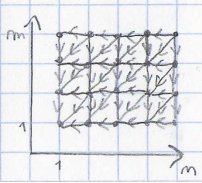
\includegraphics[]{appels.pdf}

\end{document}
